%!TEX TS-program = xelatex
%!TEX encoding = UTF-8 Unicode

\documentclass[11pt,tikz,border=1]{standalone}
\usetikzlibrary{calc,positioning}

\begin{document}
  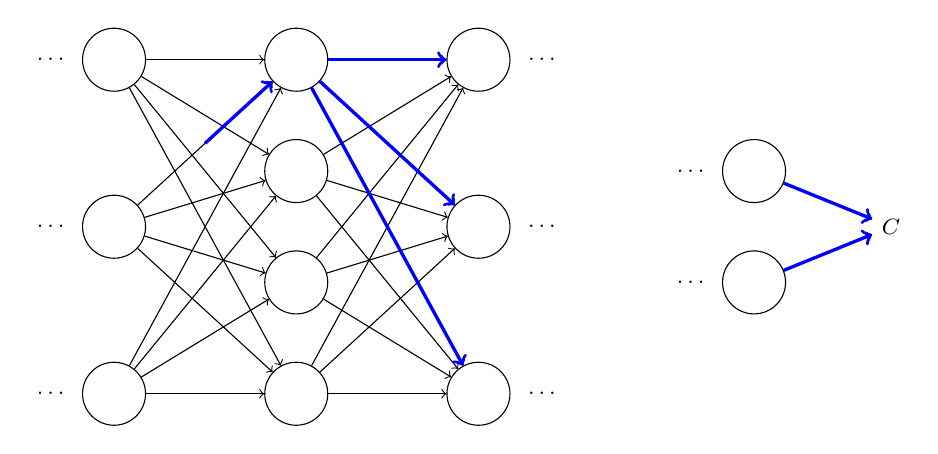
\begin{tikzpicture}[
    neuron/.style={circle,draw,inner sep=0pt,minimum size=8mm},
    font=\footnotesize
    ]

    \node(l0) [neuron] {};

    \node(m0) [neuron,right=1.5 of l0] {};
    \node(m1) [neuron,above=0.6 of m0] {};
    \node(m2) [neuron,above=0.6 of m1] {};
    \node(m3) [neuron,above=0.6 of m2] {};

    \node(l2) [neuron,left=1.5 of m3] {};

    \node(r0) [neuron,right=1.5 of m0] {};
    \node(r2) [neuron,right=1.5 of m3] {};

    \coordinate (lc) at ($(l0)!0.5!(l2)$);
    \node(l1) at (lc) [neuron] {};

    \coordinate (rc) at ($(r0)!0.5!(r2)$);
    \node(r1) at (rc) [neuron] {};

    \foreach \x in {0,1,2}
    \node(tl\x) [left=0.1 of l\x] {$\ldots$};

    \foreach \x in {0,1,2}
      \node(tr\x) [right=0.1 of r\x] {$\ldots$};

    \node (n0) [neuron,right=5 of m1] {};
    \node (n1) [neuron,right=5 of m2] {};
	  \coordinate (nc) at ($(n0)!0.5!(n1)$);
    \node (c) [right=1.5 of nc] {$C$};
    \node(tn0) [left=0.1 of n0] {$\ldots$};
    \node(tn1) [left=0.1 of n1] {$\ldots$};

	% connections:
	\foreach \x in {0,1,2}
		\foreach \y in {0,...,3}
			\draw[->] (l\x) to (m\y);

	\foreach \x in {0,...,3}
		\foreach \y in {0,1,2}
			\draw[->] (m\x) to (r\y);

    \draw[->] (n0) to (c);
    \draw[->] (n1) to (c);

    % mark:

    \coordinate (p) at ($(l1)!0.5!(m3)$);
    \draw[->,very thick,blue] (p) to (m3);
    \draw[->,very thick,blue] (m3) to (r0);
    \draw[->,very thick,blue] (m3) to (r1);
    \draw[->,very thick,blue] (m3) to (r2);
    \draw[->,very thick,blue] (n0) to (c);
    \draw[->,very thick,blue] (n1) to (c);

  \end{tikzpicture}
\end{document}
